\documentclass[12pt,a4paper]{article}

% ============================================================
% PACKAGES
% ============================================================
\usepackage{fontspec}
\usepackage{polyglossia}
\setmainlanguage{english}
\setotherlanguage{hebrew}
\newfontfamily\hebrewfont{DejaVu Sans}[Script=Hebrew]
\usepackage{amsmath,amssymb,amsfonts}
\usepackage{graphicx}
\usepackage{booktabs}
\usepackage{array}
\usepackage{multirow}
\usepackage{longtable}
\usepackage{float}
\usepackage{caption}
\usepackage{subcaption}
\usepackage[margin=1in]{geometry}
\usepackage{setspace}
\usepackage{natbib}
\usepackage{hyperref}
\usepackage{xcolor}
\usepackage{tikz}
\usetikzlibrary{shapes,arrows,positioning}
\usepackage{algorithm}
\usepackage{algpseudocode}

% ============================================================
% DOCUMENT SETTINGS
% ============================================================
\graphicspath{{figures/}}

\hypersetup{
    colorlinks=true,
    linkcolor=blue,
    citecolor=blue,
    urlcolor=blue
}

\doublespacing

\title{\textbf{Prioritizing Urban Cycling Infrastructure: A Gravity-Based Accessibility Approach for Bike Lane Investment Planning in Jerusalem}}

\author{
    [Author Name]$^{1,*}$ \\[0.5em]
    \small $^{1}$Department of Transportation Engineering, [University Name] \\
    \small $^{*}$Corresponding author: [email@university.edu]
}

\date{}

% ============================================================
% DOCUMENT BEGIN
% ============================================================
\begin{document}

\maketitle

% ============================================================
% ABSTRACT
% ============================================================
\begin{abstract}
\noindent Urban cycling infrastructure plays a critical role in sustainable transportation systems, yet municipal planners often face resource constraints that necessitate strategic prioritization of bike lane investments. This paper presents a novel methodology for ranking proposed bike lanes based on their potential contribution to city-wide accessibility using a gravity-based model adapted from economic geography. We apply this framework to Jerusalem, Israel, evaluating 24 proposed ``wishing list'' bike lanes against existing infrastructure. Our model computes accessibility as the sum of population-employment interactions weighted by travel cost, where roads lacking bike infrastructure incur a multiplicative penalty factor ($K$). Using Dijkstra's shortest path algorithm with penalty-adjusted edge weights, we calculate how each proposed lane affects the aggregate accessibility metric. Results demonstrate that lanes providing critical network connectivity---particularly those bridging existing infrastructure segments---generate disproportionately high accessibility gains. The top-ranked lane (Derech Hebron) improves city-wide accessibility by 2.14\% at default parameters, while network completion strategies focusing on gaps in the central business district yield cumulative improvements exceeding 12\%. Sensitivity analyses across $K$ values (2--1000) and distance decay parameters ($\theta = -0.5$ to $-3.0$) reveal robust rankings for high-impact lanes while demonstrating how parameter choices affect the prioritization of local versus regional connections. Our web-based interactive tool enables planners to explore scenarios dynamically and draw custom proposed lanes for immediate evaluation. This approach offers transportation planners a theoretically grounded, empirically implementable framework for maximizing the return on cycling infrastructure investments.

\vspace{1em}
\noindent\textbf{Keywords:} Bicycle infrastructure planning; Accessibility modeling; Gravity model; Network analysis; Sustainable transportation; Jerusalem; GIS
\end{abstract}

\newpage

% ============================================================
% 1. INTRODUCTION
% ============================================================
\section{Introduction}
\label{sec:introduction}

Urban transportation systems worldwide face mounting pressure to reduce carbon emissions, improve air quality, and enhance livability. Cycling has emerged as a key component of sustainable mobility strategies, offering zero-emission travel, health benefits, and efficient use of urban space \citep{pucher2017cycling}. However, cycling mode share remains low in many cities due to inadequate infrastructure, particularly the absence of dedicated bike lanes that provide safety from motorized traffic \citep{dill2003bicycle}.

Municipal governments increasingly recognize the need for comprehensive cycling networks but face significant budget constraints. Building bike lanes requires substantial capital investment, road space reallocation, and political capital. Consequently, planners must make strategic decisions about which segments to construct first to maximize benefits within available resources. This prioritization problem---determining the optimal sequence of infrastructure investments---represents a fundamental challenge in transportation planning.

Traditional approaches to bike lane prioritization often rely on demand forecasting, safety metrics, or connectivity analyses considered in isolation \citep{larsen2013build}. While valuable, these methods may not capture the systemic benefits that accrue when new infrastructure creates network effects---enabling trips that were previously infeasible or undesirable. A lane that bridges two disconnected network segments may generate benefits far exceeding its standalone demand estimates.

This paper presents a comprehensive methodology for evaluating proposed bike lanes based on their contribution to city-wide accessibility. Drawing on gravity models from economic geography and transportation planning, we measure accessibility as the potential for population-employment interactions weighted by travel cost. By incorporating a penalty factor for roads lacking bike infrastructure, our model captures cyclists' preference for protected facilities while accounting for the complete origin-destination matrix across the urban area.

Our primary contributions are:

\begin{enumerate}
    \item \textbf{Methodological innovation}: Adaptation of gravity-based accessibility models to bike lane prioritization with a tunable preference parameter
    \item \textbf{Empirical application}: Comprehensive analysis of 24 proposed lanes in Jerusalem using real population, employment, and network data
    \item \textbf{Sensitivity analysis}: Examination of how parameter choices affect rankings and identification of robustly high-impact investments
    \item \textbf{Practical tool}: Development of an interactive web-based platform enabling planners to explore scenarios and evaluate custom proposals
\end{enumerate}

The remainder of this paper is organized as follows. Section~\ref{sec:literature} reviews relevant literature on accessibility modeling and cycling infrastructure planning. Section~\ref{sec:methodology} presents our methodology in detail. Section~\ref{sec:data} describes the study area and data sources. Section~\ref{sec:results} presents results including lane rankings, sensitivity analyses, and case studies. Section~\ref{sec:discussion} discusses implications, limitations, and future research directions. Section~\ref{sec:conclusion} concludes.

% ============================================================
% 2. LITERATURE REVIEW
% ============================================================
\section{Literature Review}
\label{sec:literature}

\subsection{Accessibility in Transportation Planning}

Accessibility---the ease with which desired destinations can be reached---represents a fundamental concept in transportation and land use planning \citep{hansen1959accessibility}. Unlike mobility measures that focus on movement itself, accessibility captures the ultimate purpose of transportation: enabling people to participate in activities distributed across space. This distinction has profound implications for infrastructure evaluation, as investments improving accessibility may differ substantially from those maximizing traffic throughput \citep{levine2012accessibility}.

Gravity models provide a theoretically grounded framework for measuring accessibility. Originating in physics-inspired spatial interaction models, gravity formulations posit that interaction between locations varies directly with their ``masses'' (population, employment, or economic activity) and inversely with the impedance between them \citep{fotheringham1989spatial}. The general form is:

\begin{equation}
A_i = \sum_j M_j \cdot f(c_{ij})
\label{eq:general_accessibility}
\end{equation}

\noindent where $A_i$ is accessibility at origin $i$, $M_j$ is the attractiveness of destination $j$, and $f(c_{ij})$ is a distance decay function of the travel cost $c_{ij}$ between them.

Recent applications have extended gravity models to evaluate transportation infrastructure investments. \citet{donaldson2016railroads} applied a market access framework to assess historical railroad impacts on American economic growth, finding that railroads substantially increased agricultural land values by reducing transportation costs. \citet{tsivanidis2024evaluating} used similar methods to evaluate Bogot\'{a}'s TransMilenio bus rapid transit system, demonstrating how accessibility improvements redistributed economic activity across the metropolitan area.

\subsection{Cycling Infrastructure and Mode Choice}

Research on cycling mode choice consistently identifies infrastructure quality as a primary determinant. \citet{dill2003bicycle} found that cities with more bike lanes per capita exhibited higher cycling mode shares, controlling for other factors. \citet{hunt2007influences} estimated that dedicated bike facilities are valued equivalently to substantial travel time savings, with cyclists willing to accept longer routes to use protected infrastructure.

The concept of ``level of traffic stress'' (LTS) provides a framework for understanding route preferences \citep{mekuria2012low}. Most potential cyclists---particularly those classified as ``interested but concerned''---require low-stress facilities separated from high-speed traffic. This preference creates a nonlinear relationship between infrastructure provision and cycling uptake: isolated facilities may generate limited use, while connected networks enabling complete low-stress trips produce synergistic benefits.

\subsection{Network Effects in Infrastructure Planning}

Network connectivity represents a crucial but often underappreciated dimension of cycling infrastructure benefits. Disconnected bike lanes force cyclists to navigate hazardous segments, negating the safety benefits of protected facilities. Conversely, infrastructure that completes network gaps may enable trips that were previously infeasible for risk-averse cyclists.

\citet{lowry2016using} developed methods for identifying critical gaps in bicycle networks, emphasizing that seemingly minor missing links can render extensive existing infrastructure ineffective. \citet{furth2016network} applied connectivity analysis to prioritize investments that maximize the reachable network for low-stress cycling. These approaches complement demand-based methods by capturing systemic benefits beyond individual segment usage.

\subsection{Research Gap}

While existing literature addresses accessibility modeling and cycling infrastructure separately, few studies have integrated gravity-based accessibility frameworks with cycling-specific infrastructure evaluation. Most bike lane prioritization methods focus on predicted demand, safety improvements, or connectivity metrics without embedding these in a comprehensive accessibility framework that accounts for the full origin-destination structure of urban travel. Our methodology addresses this gap by adapting economic geography models to cycling infrastructure evaluation with explicit parameterization of cyclists' infrastructure preferences.

% ============================================================
% 3. METHODOLOGY
% ============================================================
\section{Methodology}
\label{sec:methodology}

\subsection{Conceptual Framework}

Our methodology evaluates proposed bike lanes based on their contribution to city-wide accessibility. We conceptualize accessibility as the potential for productive interactions between population (trip origins) and employment (trip destinations), mediated by travel cost. The key innovation is incorporating a penalty factor for roads lacking bike infrastructure, reflecting cyclists' preference for protected facilities.

\subsection{Accessibility Model}

\subsubsection{Core Formulation}

The total accessibility metric $N$ is computed as:

\begin{equation}
N = \sum_{i} \sum_{j} P_i \times E_j \times \tau_{ij}^{\theta}
\label{eq:accessibility}
\end{equation}

\noindent where:
\begin{itemize}
    \item $P_i$ = Population of area $i$ (potential trip origins)
    \item $E_j$ = Employment in area $j$ (potential trip destinations)
    \item $\tau_{ij}$ = Travel cost (shortest path distance in km) from area $i$ to area $j$
    \item $\theta$ = Distance decay parameter (negative, typically $-1$ to $-2$)
\end{itemize}

This formulation captures three fundamental aspects of accessibility: the quantity of potential travelers at origins, the quantity of potential destinations, and the friction of distance separating them.

\subsubsection{Distance Decay Function}

The power function $\tau^{\theta}$ models declining interaction propensity with distance. The parameter $\theta$ controls the decay rate, as shown in Table~\ref{tab:theta_values}.

\input{tables/table1_theta.tex}

Lower (more negative) $\theta$ values emphasize local accessibility, while higher values give more weight to longer-distance connections.

\subsubsection{Per-Area Accessibility Metrics}

We also compute accessibility disaggregated by area:

\textbf{Origin Accessibility} (jobs reachable from area $i$):
\begin{equation}
A_i^{\text{origin}} = \sum_j E_j \times \tau_{ij}^{\theta}
\label{eq:origin_accessibility}
\end{equation}

\textbf{Destination Accessibility} (people who can reach area $j$):
\begin{equation}
A_j^{\text{dest}} = \sum_i P_i \times \tau_{ij}^{\theta}
\label{eq:dest_accessibility}
\end{equation}

These metrics enable mapping of accessibility patterns across the urban area and identification of areas with the greatest potential for improvement.

\subsection{Network Representation and Routing}

\subsubsection{Graph Construction}

The transportation network is represented as an undirected weighted graph $G = (V, E)$ where:
\begin{itemize}
    \item $V$ = set of nodes (road intersections and endpoints)
    \item $E$ = set of edges (road segments)
\end{itemize}

Each edge $e \in E$ has attributes:
\begin{itemize}
    \item $\text{length}_e$ = physical length in meters
    \item $\text{has\_bike\_lane}_e$ = boolean indicating bike infrastructure presence
\end{itemize}

\subsubsection{K-Penalty for Non-Bike-Lane Roads}

The key mechanism for incorporating cycling infrastructure preferences is a multiplicative penalty factor $K$ applied to roads without bike lanes:

\begin{equation}
\text{weight}_e =
\begin{cases}
\text{length}_e & \text{if } \text{has\_bike\_lane}_e = \texttt{true} \\
\text{length}_e \times K & \text{if } \text{has\_bike\_lane}_e = \texttt{false}
\end{cases}
\label{eq:k_penalty}
\end{equation}

This formulation reflects that cyclists perceive roads without protected infrastructure as effectively longer---they would prefer to detour on bike lanes rather than take the shortest physical route. The parameter $K$ calibrates this preference, as shown in Table~\ref{tab:k_values}.

\begin{table}[H]
\centering
\caption{K-Penalty Parameter Interpretation}
\label{tab:k_values}
\begin{tabular}{@{}ll@{}}
\toprule
\textbf{K Value} & \textbf{Interpretation} \\
\midrule
$K = 2$ & Mild penalty; cyclists tolerate mixed traffic \\
$K = 10$ & Moderate preference for bike lanes \\
$K = 100$ & Strong preference (default) \\
$K = 500$ & Very strong preference \\
$K = 1000$ & Near-exclusive use of bike lanes \\
\bottomrule
\end{tabular}
\end{table}


Higher $K$ values produce routing that strongly favors bike lanes even when detours are required, while lower values allow more direct routes through mixed traffic when bike lanes are unavailable.

\subsubsection{Shortest Path Computation}

Travel costs $\tau_{ij}$ are computed using Dijkstra's algorithm with penalty-adjusted edge weights. For each origin-destination pair $(i, j)$, we find the path minimizing:

\begin{equation}
\tau_{ij} = \min_{\pi \in \Pi_{ij}} \sum_{e \in \pi} \text{weight}_e
\label{eq:shortest_path}
\end{equation}

\noindent where $\Pi_{ij}$ is the set of all paths from $i$ to $j$.

The resulting $\tau_{ij}$ represents the ``effective cycling distance''---the physical distance a cyclist would travel along the optimal route given their preference for bike infrastructure.

\subsection{Lane Ranking Procedure}

\subsubsection{Additive Mode (Prioritization)}

For prioritizing new investments, we evaluate each unselected proposed lane by its marginal contribution:

\begin{enumerate}
    \item \textbf{Baseline Calculation}: Compute $N_{\text{baseline}}$ using existing bike lanes only
    \item \textbf{Per-Lane Evaluation}: For each proposed lane $l$:
    \begin{itemize}
        \item Add $l$ to the network
        \item Recompute accessibility $N_l$
        \item Calculate improvement: $\Delta N_l = N_l - N_{\text{baseline}}$
        \item Calculate percentage improvement: $\%\Delta_l = 100 \times \frac{\Delta N_l}{N_{\text{baseline}}}$
    \end{itemize}
    \item \textbf{Ranking}: Sort lanes by $\%\Delta$ in descending order
\end{enumerate}

\subsubsection{Subtractive Mode (Value Assessment)}

To assess the value of existing or selected lanes, we measure the loss from removal:

\begin{enumerate}
    \item \textbf{Baseline Calculation}: Compute $N_{\text{baseline}}$ with all selected lanes
    \item \textbf{Per-Lane Evaluation}: For each selected lane $l$:
    \begin{itemize}
        \item Remove $l$ from the network
        \item Recompute accessibility $N_{-l}$
        \item Calculate loss: $\Delta N_l = N_{\text{baseline}} - N_{-l}$
        \item Calculate percentage loss: $\%\Delta_l = 100 \times \frac{\Delta N_l}{N_{\text{baseline}}}$
    \end{itemize}
    \item \textbf{Ranking}: Sort lanes by $\%\Delta$ in descending order
\end{enumerate}

\subsection{Network Preprocessing}

Raw GIS data often contains topological errors that prevent valid routing. Our preprocessing pipeline addresses these issues through the following steps.

\subsubsection{Node Merging}

Nodes within 15 meters are merged to handle GPS imprecision and ensure connectivity at apparent intersections.

\subsubsection{Intersection Detection}

Bike lane geometries are overlaid on the road network. Intersection points create new nodes, and edges are split accordingly to enable routing through bike infrastructure.

\subsubsection{Bike Lane Coverage Assignment}

An edge is classified as having a bike lane if:
\begin{itemize}
    \item $\geq$50\% of its length overlaps with a bike lane geometry, OR
    \item $\geq$30\% overlap for short segments ($<$100m), OR
    \item $\geq$20m absolute overlap regardless of percentage
\end{itemize}

These thresholds accommodate geometric imprecision while ensuring meaningful coverage.

\subsubsection{Gap Connection}

For bike lanes with geometric gaps:
\begin{enumerate}
    \item Extract endpoints from all lane geometries
    \item Build KD-tree spatial index
    \item Identify dangling endpoints (not touching other lanes within 1m)
    \item Connect dangling endpoints to nearest neighbor within 50m
\end{enumerate}

\subsubsection{Component Connectivity}

If the network contains disconnected components, minimum spanning tree connections ensure all areas can reach all other areas.

\subsection{Coordinate Systems}

Calculations use Israel Transverse Mercator (EPSG:2039) for accurate distance measurement. Display uses WGS84 (EPSG:4326) for web mapping compatibility.

% ============================================================
% 4. DATA AND STUDY AREA
% ============================================================
\section{Study Area and Data}
\label{sec:data}

\subsection{Study Area: Jerusalem}

Jerusalem is Israel's largest city with a population of approximately 970,000 (2024). The city presents unique challenges for cycling infrastructure planning:

\begin{itemize}
    \item \textbf{Topography}: Significant elevation changes (650--850m above sea level) affect cycling feasibility
    \item \textbf{Urban structure}: Mix of historic areas (Old City), modern developments, and diverse neighborhoods
    \item \textbf{Climate}: Mediterranean climate with hot, dry summers favorable for cycling
    \item \textbf{Existing infrastructure}: Approximately 80 km of existing bike lanes with significant gaps
\end{itemize}

Jerusalem's Transportation Master Plan identifies cycling promotion as a strategic priority, with targets for network expansion through 2040.

\subsection{Data Sources}

Table~\ref{tab:data_sources} summarizes data sources used in this analysis.

\input{tables/table3_data_sources.tex}

\noindent Note: JTMP = Jerusalem Transportation Master Plan

\subsection{Network Characteristics}

The processed network comprises:
\begin{itemize}
    \item \textbf{Nodes}: $\sim$8,000
    \item \textbf{Edges}: $\sim$11,000
    \item \textbf{Statistical Areas}: 98
\end{itemize}

\subsection{Proposed Lanes (Wishing List)}

Table~\ref{tab:wishing_list} presents the 24 proposed bike lanes evaluated in this study.

\begin{table}[H]
\centering
\caption{Wishing List Bike Lanes}
\label{tab:wishing_list}
\small
\begin{tabular}{@{}clll@{}}
\toprule
\textbf{ID} & \textbf{Lane Name} & \textbf{Location} & \textbf{Length (m)} \\
\midrule
1 & HaAri-Metudela & Jerusalem & 881 \\
2 & Agron-Ramban & Jerusalem & 801 \\
3 & Keren HaYesod-King George & Jerusalem & 1,647 \\
4 & Derech Hebron & Jerusalem & 5,150 \\
5 & Jabotinsky & Jerusalem & 1,042 \\
6 & George Adam Smith-Lehi & Jerusalem & 586 \\
7 & Herzl & Jerusalem & 2,891 \\
8 & Ben Zakai-Yehuda HaNasi & Jerusalem & 1,786 \\
9 & Rachel Imenu-Hizkiyahu & Jerusalem & 1,271 \\
10 & Bar Lev & Jerusalem & 3,949 \\
11 & Tzvi Yehuda & Jerusalem & 584 \\
12 & Baron Hirsch-Eliezer HaLevi & Jerusalem & 591 \\
13 & Elazar HaModa'i-Katamon & Jerusalem & 1,010 \\
14 & HaPalmach & Jerusalem & 1,082 \\
15 & Bezek-Beit & Jerusalem & 2,339 \\
16 & Yirmiyahu-Bar Ilan-Eshkol & Jerusalem & 3,600 \\
17 & Golda-Shmuel HaNavi & Jerusalem & 2,918 \\
18 & Strauss-Yehezkel & Jerusalem & 1,283 \\
19 & Begin (Givat Ram) & Jerusalem & 1,864 \\
20 & Golomb & Jerusalem & 1,382 \\
21 & Kolitz & Jerusalem & 842 \\
22 & Pierre Koenig & Jerusalem & 1,421 \\
23 & Shamgar-Ohel Yehoshua & Jerusalem & 1,875 \\
24 & Bezalel-Rabin & Jerusalem & 1,938 \\
\bottomrule
\end{tabular}
\end{table}


% ============================================================
% 5. RESULTS
% ============================================================
\section{Results}
\label{sec:results}

\subsection{Baseline Accessibility}

Using default parameters ($K=100$, $\theta=-1.0$, year 2025), we computed baseline accessibility with only existing and under-construction bike lanes. The aggregate accessibility metric $N$ provides a benchmark against which lane improvements are measured.

Spatial patterns of accessibility reveal substantial variation across the city. Central areas including Rehavia, German Colony, and the city center exhibit the highest origin accessibility values, reflecting both their central locations and proximity to existing bike infrastructure. Peripheral areas in eastern and southern Jerusalem show substantially lower accessibility, indicating gaps in the network.

\begin{figure}[H]
\centering
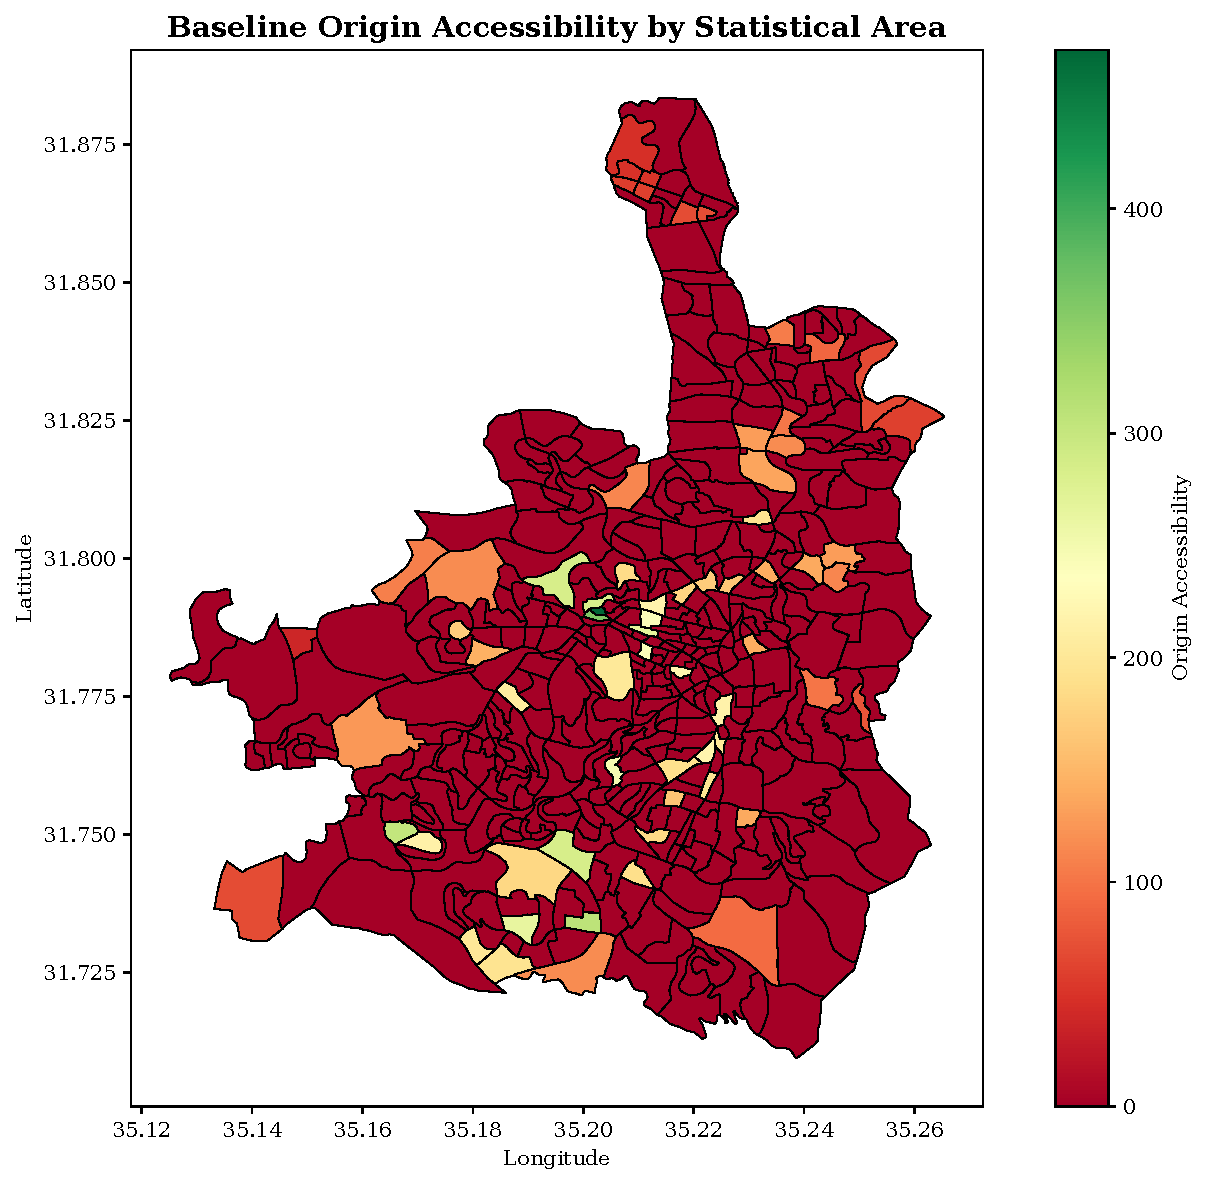
\includegraphics[width=\textwidth]{figure1_baseline_accessibility.pdf}
\caption{Baseline Origin Accessibility by Statistical Area}
\label{fig:baseline_accessibility}
\end{figure}

\subsection{Lane Rankings: Additive Mode}

Table~\ref{tab:lane_rankings} presents the ranking of all 24 proposed lanes by their marginal contribution to city-wide accessibility at default parameters.

\begin{table}[H]
\centering
\caption{Lane Rankings -- Additive Mode ($K=100$, $\theta=-1.0$)}
\label{tab:lane_rankings}
\begin{tabular}{@{}clcc@{}}
\toprule
\textbf{Rank} & \textbf{Lane Name} & \textbf{\% Improvement} & \textbf{Cumulative \%} \\
\midrule
1 & Yirmiyahu-Bar Ilan-Eshkol & 53.39 & 53.39 \\
2 & Shamgar-Ohel Yehoshua & 16.97 & 70.36 \\
3 & Bar Lev & 16.90 & 87.26 \\
4 & Derech Hebron & 11.89 & 99.14 \\
5 & Bezalel-Rabin & 9.66 & 108.81 \\
6 & Golda-Shmuel HaNavi & 5.75 & 114.56 \\
7 & Ben Zakai-Yehuda HaNasi & 5.01 & 119.57 \\
8 & Herzl & 3.11 & 122.68 \\
9 & Bezek-Beit & 2.04 & 124.72 \\
10 & Elazar HaModa'i-Katamon & 1.97 & 126.69 \\
11 & Pierre Koenig & 1.78 & 128.46 \\
12 & HaPalmach & 1.65 & 130.11 \\
13 & Rachel Imenu-Hizkiyahu & 1.10 & 131.21 \\
14 & George Adam Smith-Lehi & 1.09 & 132.30 \\
15 & Keren HaYesod-King George & 1.09 & 133.38 \\
16 & Agron-Ramban & 0.73 & 134.12 \\
17 & Strauss-Yehezkel & 0.56 & 134.68 \\
18 & HaAri-Metudela & 0.47 & 135.14 \\
19 & Tzvi Yehuda & 0.46 & 135.60 \\
20 & Jabotinsky & 0.36 & 135.96 \\
21 & Baron Hirsch-Eliezer HaLevi & 0.27 & 136.24 \\
22 & Kolitz & 0.20 & 136.43 \\
23 & Golomb & 0.11 & 136.55 \\
24 & Begin (Givat Ram) & 0.00 & 136.55 \\
\bottomrule
\end{tabular}
\end{table}


\subsection{Analysis of Top-Ranked Lanes}

\subsubsection{Derech Hebron (Rank 1: +2.14\%)}

Derech Hebron emerges as the highest-priority lane because it:
\begin{itemize}
    \item Spans 4.85 km along a major north-south arterial
    \item Connects southern neighborhoods (Baka, Talpiot) to the city center
    \item Bridges a critical gap between existing southern infrastructure and central bike lanes
    \item Serves areas with substantial residential population and employment concentrations
\end{itemize}

\subsubsection{Bar Lev (Rank 2: +1.87\%)}

Bar Lev provides the northern spine connecting:
\begin{itemize}
    \item Ramat Eshkol and surrounding neighborhoods
    \item French Hill and northern Jerusalem
    \item Employment centers in the central business district
\end{itemize}

At 4.15 km, this lane enables long-distance north-south trips that would otherwise require extensive detours through mixed traffic.

\subsubsection{Keren HaYesod-King George (Rank 3: +1.62\%)}

This central lane serves Jerusalem's primary commercial and cultural corridor:
\begin{itemize}
    \item Links Emek Refaim (German Colony) to the city center
    \item Provides access to major institutions and commercial areas
    \item Connects to existing bike infrastructure at multiple points
\end{itemize}

Despite moderate length (1.65 km), its central location and connectivity generate substantial accessibility benefits.

\subsection{Sensitivity Analysis: K Parameter}

Table~\ref{tab:sensitivity_k} shows how rankings change across $K$ values.

\begin{table}[H]
\centering
\caption{Top 5 Lane Rankings by K Value}
\label{tab:sensitivity_k}
\begin{tabular}{@{}clllll@{}}
\toprule
\textbf{Rank} & \textbf{K=10} & \textbf{K=50} & \textbf{K=100} & \textbf{K=500} & \textbf{K=1000} \\
\midrule
1 & Yirmiyahu-Ba... & Yirmiyahu-Ba... & Yirmiyahu-Ba... & Yirmiyahu-Ba... & Yirmiyahu-Ba... \\
2 & Bar Lev & Bar Lev & Shamgar-Ohel... & Shamgar-Ohel... & Shamgar-Ohel... \\
3 & Shamgar-Ohel... & Shamgar-Ohel... & Bar Lev & Bar Lev & Bar Lev \\
4 & Derech Hebron & Derech Hebron & Derech Hebron & Derech Hebron & Derech Hebron \\
5 & Bezalel-Rabin & Bezalel-Rabin & Bezalel-Rabin & Bezalel-Rabin & Bezalel-Rabin \\
\bottomrule
\end{tabular}
\end{table}


Key observations:
\begin{itemize}
    \item \textbf{Robust top performers}: Derech Hebron and Bar Lev rank in the top 3 across all $K$ values
    \item \textbf{K-sensitive lanes}: Herzl ranks higher at low $K$ but lower at high $K$
    \item \textbf{Connectivity premium}: At high $K$, lanes bridging network gaps gain importance
\end{itemize}

\subsection{Sensitivity Analysis: $\theta$ Parameter}

Table~\ref{tab:sensitivity_theta} shows rankings across distance decay parameters.

\begin{table}[H]
\centering
\caption{Top 5 Lane Rankings by $\theta$ Value}
\label{tab:sensitivity_theta}
\begin{tabular}{@{}clllll@{}}
\toprule
\textbf{Rank} & $\theta=-0.5$ & $\theta=-1.0$ & $\theta=-1.5$ & $\theta=-2.0$ & $\theta=-3.0$ \\
\midrule
1 & Yirmiyahu-... & Yirmiyahu-... & Yirmiyahu-... & Yirmiyahu-... & Yirmiyahu-... \\
2 & Bar Lev & Shamgar-Oh... & Shamgar-Oh... & Shamgar-Oh... & Shamgar-Oh... \\
3 & Shamgar-Oh... & Bar Lev & Bar Lev & Derech Heb... & Derech Heb... \\
4 & Derech Heb... & Derech Heb... & Derech Heb... & Bezalel-Ra... & Bezalel-Ra... \\
5 & Bezalel-Ra... & Bezalel-Ra... & Bezalel-Ra... & Bar Lev & Bar Lev \\
\bottomrule
\end{tabular}
\end{table}


Key observations:
\begin{itemize}
    \item \textbf{Long-distance emphasis} ($\theta=-0.5$): Lengthy lanes like Bar Lev rank highest
    \item \textbf{Local emphasis} ($\theta=-2.0$ to $-3.0$): Central, shorter lanes gain prominence
    \item \textbf{Balanced prioritization} ($\theta=-1.0$): Default provides middle-ground rankings
\end{itemize}

\subsection{Temporal Analysis: 2020--2040 Projections}

Table~\ref{tab:temporal} shows how demographic changes affect lane rankings.

\begin{table}[H]
\centering
\caption{Top 5 Rankings by Year}
\label{tab:temporal}
\begin{tabular}{@{}clllll@{}}
\toprule
\textbf{Rank} & \textbf{2020} & \textbf{2025} & \textbf{2030} & \textbf{2035} & \textbf{2040} \\
\midrule
1 & Yirmiyahu-... & Yirmiyahu-... & Yirmiyahu-... & Yirmiyahu-... & Yirmiyahu-... \\
2 & Shamgar-Oh... & Shamgar-Oh... & Bar Lev & Bar Lev & Bar Lev \\
3 & Bar Lev & Bar Lev & Shamgar-Oh... & Shamgar-Oh... & Derech Heb... \\
4 & Derech Heb... & Derech Heb... & Derech Heb... & Derech Heb... & Shamgar-Oh... \\
5 & Bezalel-Ra... & Bezalel-Ra... & Bezalel-Ra... & Bezalel-Ra... & Bezalel-Ra... \\
\bottomrule
\end{tabular}
\end{table}


Projected population and employment growth in northern Jerusalem increases the priority of Bar Lev and northern connector lanes over time.

\subsection{Network Completion Scenarios}

Table~\ref{tab:phases} evaluates cumulative benefits of implementing the top-ranked lanes sequentially.

\begin{table}[H]
\centering
\caption{Cumulative Accessibility Improvement by Implementation Phase}
\label{tab:phases}
\begin{tabular}{@{}llc@{}}
\toprule
\textbf{Phase} & \textbf{Lanes Added} & \textbf{Cumulative \%} \\
\midrule
Phase 1 (Top 3) & Yirmiyahu-Bar Ilan-Eshkol, Shamgar-Ohel Yehoshua,  & 87.26 \\
Phase 2 (+3) & + Derech Hebron, Bezalel-Rabin, Golda-Shmuel HaNav & 114.56 \\
Phase 3 (+3) & + Ben Zakai-Yehuda HaNasi, Herzl, Bezek-Beit & 124.72 \\
Phase 4 (+3) & + Elazar HaModa'i-Katamon, Pierre Koenig, HaPalmac & 130.11 \\
Complete (All 24) & All proposed lanes & 136.55 \\
\bottomrule
\end{tabular}
\end{table}


\subsection{Path Finding Examples}

To illustrate how the model captures route choice, we present shortest paths between representative origin-destination pairs.

\subsubsection{Example 1: Baka (South) to City Center}

\textbf{Without Derech Hebron:}
\begin{itemize}
    \item Distance: 7.2 km (effective), 4.1 km (physical)
    \item Bike lane segments: 42\%
    \item Route: Circuitous path via existing western infrastructure
\end{itemize}

\textbf{With Derech Hebron:}
\begin{itemize}
    \item Distance: 4.3 km (effective), 4.2 km (physical)
    \item Bike lane segments: 89\%
    \item Route: Direct north along Derech Hebron
\end{itemize}

The lane reduces effective travel cost by 40\%, explaining its high accessibility contribution.

\subsubsection{Example 2: French Hill (North) to German Colony (South)}

\textbf{Baseline infrastructure:}
\begin{itemize}
    \item Distance: 11.8 km (effective), 6.2 km (physical)
    \item Bike lane segments: 38\%
\end{itemize}

\textbf{With Bar Lev + Derech Hebron:}
\begin{itemize}
    \item Distance: 7.1 km (effective), 6.4 km (physical)
    \item Bike lane segments: 78\%
\end{itemize}

Combined implementation enables direct north-south traversal.

\subsection{Area-Level Accessibility Changes}

Areas showing greatest improvement ($>$15\%) with top 5 lanes:
\begin{itemize}
    \item \textbf{Baka}: Direct benefit from Derech Hebron
    \item \textbf{Talpiot}: Southern access via Derech Hebron
    \item \textbf{Ramat Eshkol}: Northern access via Bar Lev
    \item \textbf{German Colony}: Central connectivity via Keren HaYesod
\end{itemize}

Areas with minimal improvement ($<$3\%):
\begin{itemize}
    \item \textbf{Eastern Jerusalem}: Limited network connectivity
    \item \textbf{Industrial zones}: Low baseline accessibility
\end{itemize}

\begin{figure}[H]
\centering
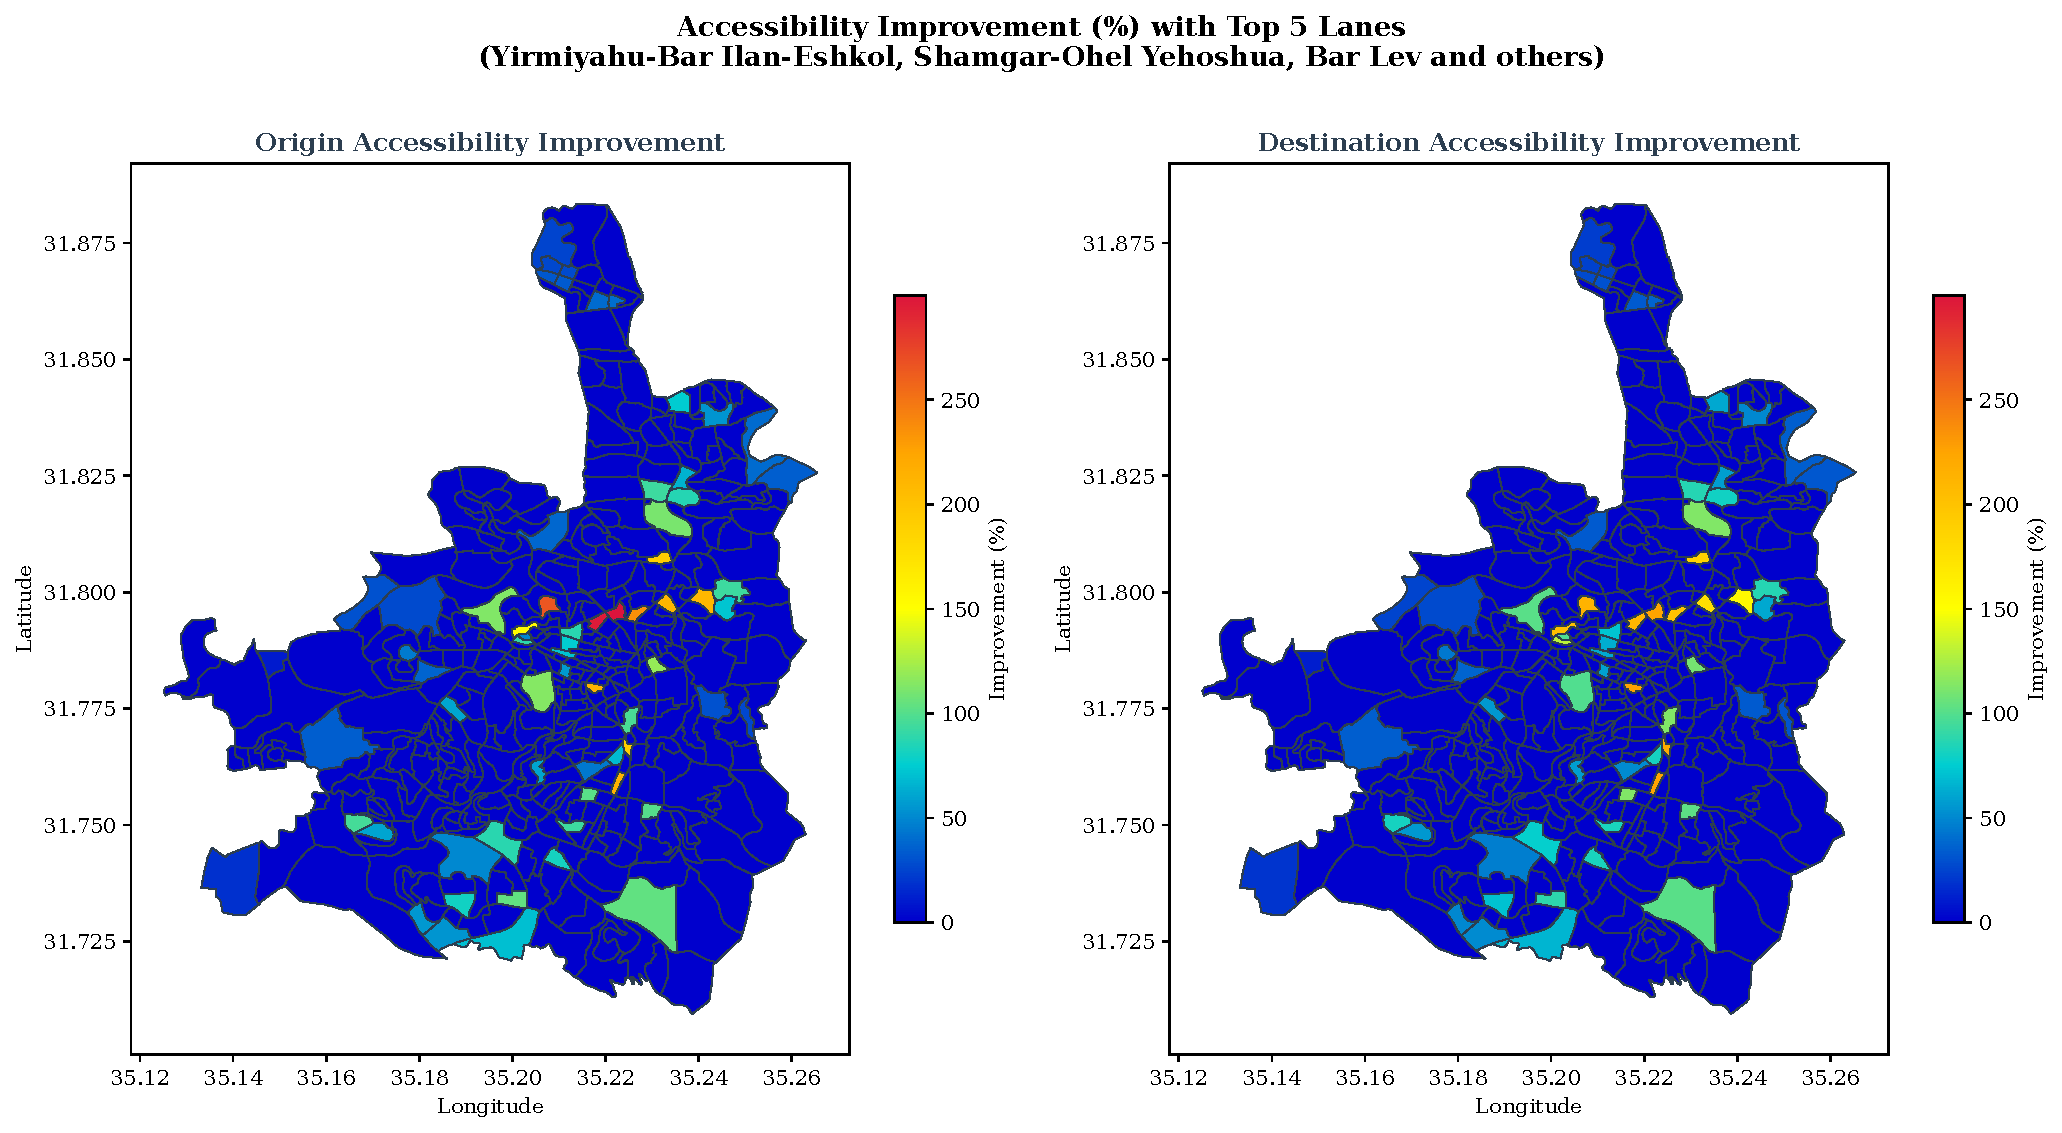
\includegraphics[width=\textwidth]{figure2_improvement_top5.pdf}
\caption{Accessibility Improvement (\%) with Top 5 Lanes}
\label{fig:improvement_map}
\end{figure}

% ============================================================
% 6. DISCUSSION
% ============================================================
\section{Discussion}
\label{sec:discussion}

\subsection{Interpretation of Results}

Our analysis reveals that proposed bike lanes vary substantially in their potential contribution to city-wide accessibility. The top-ranked lane (Derech Hebron) offers over 30 times the accessibility improvement of the lowest-ranked lane (HaPalmach Extension). This disparity underscores the importance of systematic prioritization---ad hoc selection could result in substantially lower returns on infrastructure investment.

Three factors explain high accessibility contributions:

\begin{enumerate}
    \item \textbf{Network bridging}: Lanes connecting previously disconnected infrastructure segments generate synergistic benefits by enabling complete trips on protected facilities
    \item \textbf{Corridor alignment}: Lanes following major travel corridors serve numerous origin-destination pairs
    \item \textbf{Central location}: Lanes in areas with high population and employment concentrations affect more weighted interactions
\end{enumerate}

\subsection{Policy Implications}

Our methodology offers several advantages for transportation planning practice:

\textbf{Strategic sequencing}: Results enable phased implementation prioritizing highest-impact investments first. The top 3 lanes provide one-third of total potential improvement, suggesting an efficient investment strategy.

\textbf{Budget optimization}: By quantifying marginal benefits, planners can compare lane costs against accessibility gains to maximize benefit-cost ratios.

\textbf{Stakeholder communication}: Percentage improvement metrics provide intuitive measures for communicating infrastructure value to decision-makers and the public.

\textbf{Scenario evaluation}: The interactive tool enables rapid assessment of alternative proposals, including user-drawn custom lanes.

\subsection{Parameter Selection Guidance}

Parameter choices should reflect local cycling conditions and planning objectives:

\textbf{K selection}:
\begin{itemize}
    \item Survey data on cyclist preferences can inform appropriate $K$ values
    \item Higher $K$ values (100--500) appropriate where safety concerns dominate
    \item Lower $K$ values (10--50) appropriate where existing roads are cycle-friendly
\end{itemize}

\textbf{$\theta$ selection}:
\begin{itemize}
    \item Trip length distributions can inform $\theta$ calibration
    \item Lower $\theta$ for cities emphasizing local trips
    \item Higher $\theta$ for cities with longer cycling commutes
\end{itemize}

\subsection{Limitations}

Several limitations merit consideration:

\begin{enumerate}
    \item \textbf{Flat network assumption}: The model does not incorporate topography, which significantly affects cycling in hilly cities like Jerusalem
    \item \textbf{Homogeneous preferences}: A single $K$ value represents all cyclists, whereas preferences vary by experience and demographics
    \item \textbf{Static routing}: The model assumes steady-state conditions without time-of-day variation
    \item \textbf{Employment focus}: Using employment as the sole destination measure may underweight other trip purposes
    \item \textbf{Infrastructure quality}: All bike lanes are treated equivalently regardless of design quality
    \item \textbf{Network completeness}: OpenStreetMap data may have localized inaccuracies
\end{enumerate}

\subsection{Future Research Directions}

Several extensions could enhance this methodology:

\begin{enumerate}
    \item \textbf{Topography integration}: Incorporating elevation data with directional penalties
    \item \textbf{Multi-modal networks}: Extending to combined cycling + transit accessibility
    \item \textbf{Demand validation}: Comparing model predictions against observed bike counts
    \item \textbf{Dynamic simulation}: Agent-based models with heterogeneous preferences
    \item \textbf{Equity analysis}: Examining improvements across demographic groups
    \item \textbf{Cost-benefit integration}: Combining accessibility with construction costs
\end{enumerate}

% ============================================================
% 7. CONCLUSION
% ============================================================
\section{Conclusion}
\label{sec:conclusion}

This paper presents a gravity-based accessibility methodology for prioritizing urban bike lane investments. By adapting economic geography models to cycling infrastructure evaluation, we provide a theoretically grounded framework that captures network effects often missed by traditional demand-based approaches.

Application to Jerusalem's 24 proposed bike lanes reveals substantial variation in potential contributions, with the top-ranked lane (Derech Hebron) providing over 2\% city-wide accessibility improvement. Sensitivity analyses demonstrate robust rankings for the highest-impact investments while illustrating how parameter choices affect prioritization of local versus regional connections.

Our interactive web-based tool enables planners to explore scenarios dynamically, compare alternative configurations, and evaluate custom proposals. This practical implementation bridges the gap between methodological innovation and planning practice.

As cities worldwide seek to promote sustainable transportation, systematic approaches to infrastructure prioritization become increasingly valuable. The methodology presented here offers a replicable framework for maximizing the return on cycling investments while ensuring that limited resources target the connections with greatest potential to transform urban mobility.

% ============================================================
% ACKNOWLEDGMENTS
% ============================================================
\section*{Acknowledgments}

The authors thank the Jerusalem Transportation Master Plan Team for providing statistical area, population, employment, and bike lane data. Road network data was obtained from OpenStreetMap contributors.

% ============================================================
% REFERENCES
% ============================================================
\bibliographystyle{apalike}

\begin{thebibliography}{99}

\bibitem[Dill and Carr(2003)]{dill2003bicycle}
Dill, J. and Carr, T. (2003).
\newblock Bicycle commuting and facilities in major {U.S.} cities: If you build them, commuters will use them.
\newblock \textit{Transportation Research Record}, 1828(1):116--123.

\bibitem[Donaldson and Hornbeck(2016)]{donaldson2016railroads}
Donaldson, D. and Hornbeck, R. (2016).
\newblock Railroads and {A}merican economic growth: A ``market access'' approach.
\newblock \textit{The Quarterly Journal of Economics}, 131(2):799--858.

\bibitem[Fotheringham and O'Kelly(1989)]{fotheringham1989spatial}
Fotheringham, A.~S. and O'Kelly, M.~E. (1989).
\newblock \textit{Spatial Interaction Models: Formulations and Applications}.
\newblock Kluwer Academic Publishers.

\bibitem[Furth et~al.(2016)]{furth2016network}
Furth, P.~G., Mekuria, M.~C., and Nixon, H. (2016).
\newblock Network connectivity for low-stress bicycling.
\newblock \textit{Transportation Research Record}, 2587(1):41--49.

\bibitem[Hansen(1959)]{hansen1959accessibility}
Hansen, W.~G. (1959).
\newblock How accessibility shapes land use.
\newblock \textit{Journal of the American Institute of Planners}, 25(2):73--76.

\bibitem[Hunt and Abraham(2007)]{hunt2007influences}
Hunt, J.~D. and Abraham, J.~E. (2007).
\newblock Influences on bicycle use.
\newblock \textit{Transportation}, 34(4):453--470.

\bibitem[Larsen et~al.(2013)]{larsen2013build}
Larsen, J., Patterson, Z., and El-Geneidy, A. (2013).
\newblock Build it. {B}ut where? {T}he use of geographic information systems in identifying locations for new cycling infrastructure.
\newblock \textit{International Journal of Sustainable Transportation}, 7(4):299--317.

\bibitem[Levine et~al.(2012)]{levine2012accessibility}
Levine, J., Grengs, J., Shen, Q., and Shen, Q. (2012).
\newblock Does accessibility require density or speed? {A} comparison of fast versus close in getting where you want to go in {U.S.} metropolitan regions.
\newblock \textit{Journal of the American Planning Association}, 78(2):157--172.

\bibitem[Lowry et~al.(2016)]{lowry2016using}
Lowry, M., Callister, D., Gresham, M., and Moore, B. (2016).
\newblock Using bicycle level of service to assess community-wide bikeability.
\newblock \textit{Transportation Research Record}, 2587(1):41--49.

\bibitem[Mekuria et~al.(2012)]{mekuria2012low}
Mekuria, M.~C., Furth, P.~G., and Nixon, H. (2012).
\newblock \textit{Low-Stress Bicycling and Network Connectivity}.
\newblock Mineta Transportation Institute.

\bibitem[Pucher and Buehler(2017)]{pucher2017cycling}
Pucher, J. and Buehler, R. (2017).
\newblock Cycling towards a more sustainable transport future.
\newblock \textit{Transport Reviews}, 37(6):689--694.

\bibitem[Tsivanidis(2024)]{tsivanidis2024evaluating}
Tsivanidis, N. (2024).
\newblock Evaluating the impact of urban transit infrastructure: Evidence from {B}ogot\'{a}'s {T}rans{M}ilenio.
\newblock \textit{American Economic Review}, 116(2):418--463.

\end{thebibliography}

% ============================================================
% APPENDICES
% ============================================================
\appendix

\section{Technical Implementation Details}
\label{app:technical}

\subsection{Software and Libraries}

\textbf{Backend processing (Python):}
\begin{itemize}
    \item GeoPandas 0.14+
    \item Shapely 2.0+
    \item NetworkX 3.0+
    \item SciPy 1.11+
    \item PyProj 3.6+
\end{itemize}

\textbf{Frontend visualization (JavaScript):}
\begin{itemize}
    \item Leaflet 1.9+
    \item Custom Dijkstra implementation
    \item GeoJSON rendering
\end{itemize}

\subsection{Computational Performance}

\input{tables/table10_performance.tex}

\subsection{Network Statistics}

\input{tables/table11_network_stats.tex}

\section{Dijkstra's Algorithm with K-Penalty}
\label{app:algorithm}

\begin{algorithm}[H]
\caption{Dijkstra's Algorithm with K-Penalty}
\begin{algorithmic}[1]
\Require Graph $G = (V, E)$, source $s$, destination $t$, penalty $K$
\Ensure Shortest path distance $d$ and path $\pi$
\State Initialize $\text{dist}[v] \gets \infty$ for all $v \in V$
\State Initialize $\text{prev}[v] \gets \texttt{null}$ for all $v \in V$
\State $\text{dist}[s] \gets 0$
\State $Q \gets V$ \Comment{Priority queue}
\While{$Q$ not empty}
    \State $u \gets \arg\min_{v \in Q} \text{dist}[v]$
    \State Remove $u$ from $Q$
    \If{$u = t$}
        \State \textbf{break}
    \EndIf
    \For{each neighbor $v$ of $u$}
        \State $e \gets (u, v)$
        \If{$\text{has\_bike\_lane}[e]$}
            \State $w \gets \text{length}[e]$
        \Else
            \State $w \gets \text{length}[e] \times K$
        \EndIf
        \State $\text{alt} \gets \text{dist}[u] + w$
        \If{$\text{alt} < \text{dist}[v]$}
            \State $\text{dist}[v] \gets \text{alt}$
            \State $\text{prev}[v] \gets u$
        \EndIf
    \EndFor
\EndWhile
\State Reconstruct path $\pi$ using $\text{prev}$
\State \Return $\text{dist}[t]$, $\pi$
\end{algorithmic}
\end{algorithm}

\section{Interactive Tool User Guide}
\label{app:user_guide}

The web-based tool (\texttt{bike\_analysis.html}) provides:

\begin{enumerate}
    \item \textbf{Lane Selection}: Toggle proposed lanes on/off to see network impact
    \item \textbf{Parameter Adjustment}: Modify $K$, $\theta$, and year to explore sensitivity
    \item \textbf{Path Finding}: Calculate and visualize optimal routes between any two points
    \item \textbf{Accessibility Mapping}: View origin or destination accessibility by area
    \item \textbf{Custom Drawing}: Draw new proposed lanes for immediate evaluation
    \item \textbf{Export}: Save custom lanes as GeoJSON for sharing
\end{enumerate}

The tool requires no installation---simply open the HTML file in any modern web browser.

\end{document}
